%!TEX program = lualatex
% Unofficial University of Cambridge Poster Template
% https://github.com/andiac/gemini-cam
% a fork of https://github.com/anishathalye/gemini
% also refer to https://github.com/k4rtik/uchicago-poster

\documentclass[final]{beamer}

% ====================
% Packages
% ====================

\usepackage[T1]{fontenc}
\usepackage{lmodern}
\usepackage[orientation=portrait,size=a0,scale=1.06]{beamerposter}
\usetheme{gemini}
\usecolortheme{nott}
\usepackage{graphicx}
\usepackage{booktabs}
\usepackage[numbers]{natbib} % o [authoryear] según prefieras
\usepackage{tikz}
\usepackage{pgfplots}
\pgfplotsset{compat=1.14}
\usepackage{anyfontsize}

\providecommand{\abs}[1]{\left|#1\right|}
\providecommand{\norm}[1]{\left\|#1\right\|}


% ====================
% Lengths
% ====================

% If you have N columns, choose \sepwidth and \colwidth such that
% (N+1)*\sepwidth + N*\colwidth = \paperwidth
\newlength{\sepwidth}
\newlength{\colwidth}
\setlength{\sepwidth}{0.025\paperwidth}
\setlength{\colwidth}{0.45\paperwidth}

\newcommand{\separatorcolumn}{\begin{column}{\sepwidth}\end{column}}

% ====================
% Title
% ====================

\title{Models of the universe from differential geometry.}

\author{Andrés David Cadena Simons}

\institute[shortinst]{Departamento de Matemáticas, Universidad Nacional de Colombia sede Bogotá.}

% ====================
% Footer (optional)
% ====================

\footercontent{
  Geometría Diferencial --- 2025 \hfill
  \href{mailto:acadenas@unal.edu.co}{acadenas@unal.edu.co}}
% (can be left out to remove footer)


% ====================
% Logo (optional)
% ====================

% use this to include logos on the left and/or right side of the header:
\logoright{\hspace{-20ex}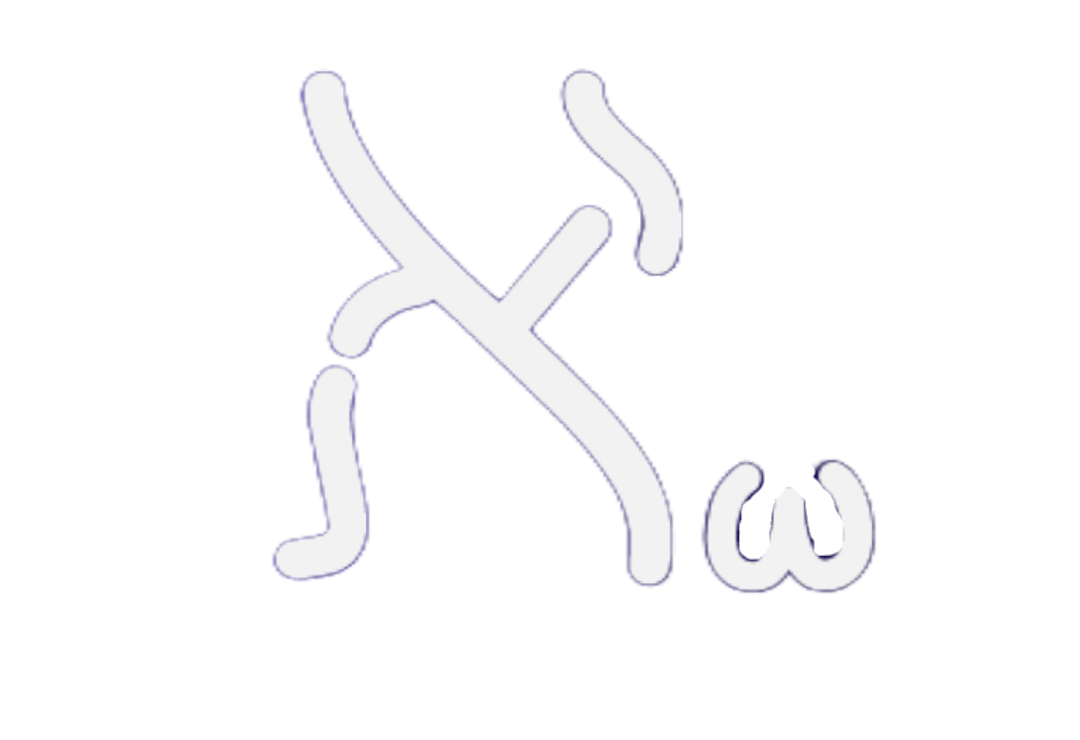
\includegraphics[height=6cm]{logos/alepth.png}}
\logoleft{\hspace{20ex}
\includegraphics[height=6cm]{logos/logo.png}}

% ====================
% Body
% ====================

\begin{document}

% Refer to https://github.com/k4rtik/uchicago-poster
% logo: https://www.cam.ac.uk/brand-resources/about-the-logo/logo-downloads
% \addtobeamertemplate{headline}{}
% {
%     \begin{tikzpicture}[remember picture,overlay]
%       \node [anchor=north west, inner sep=3cm] at ([xshift=-2.5cm,yshift=1.75cm]current page.north west)
%       {\includegraphics[height=7cm]{logos/unott-logo.eps}}; 
%     \end{tikzpicture}
% }

\begin{frame}[t]
\begin{columns}[t]
\separatorcolumn

\begin{column}{\colwidth}

  \begin{block}{Abstract}
    The document provides a clear and accessible introduction to the idea that gravity is a manifestation of spacetime curvature, as proposed by Einstein in his theory of general relativity.
    \begin{enumerate}
      \item Geodesics and curvature: It explains that the natural path of objects in curved spacetime is a geodesic, which generalizes the concept of a straight line. On curved surfaces like a sphere, geodesics are great circles.
      \item Gravity as geometry: Instead of viewing gravity as an instantaneous force (as in Newtonian theory), Einstein proposed that objects follow the curvature of spacetime shaped by the presence of matter. An analogy with an elastic membrane deformed by billiard balls is used to illustrate this idea.
      \item Models of the universe: Three types of universe are presented depending on their curvature:
      \begin{enumerate}
        \item Flat (zero curvature).
        \item Spherical (positive curvature, closed universe).
        \item Hyperbolic (negative curvature, open universe).\\
          The sum of the angles in a triangle varies with the type of curvature.
      \end{enumerate}
    \end{enumerate}
    \item Escape velocity and black holes: The concept of escape velocity is introduced as the minimum needed to break free from a gravitational field. If this velocity equals the speed of light, a black hole forms. The Schwarzschild radius is derived from this idea, showing its dependence on the object's mass.
  \end{block}

  \begin{block}{Introduction}
    Since ancient times, humans have wondered about the nature of the universe and the forces that govern the motion of celestial bodies. Newton's theory of gravity provided an effective explanation for centuries: an instantaneous force of attraction between masses. However, in the early 20th century, Albert Einstein revolutionized our understanding by proposing that gravity is not a force, but a manifestation of the curvature of spacetime caused by the presence of matter and energy.\\
    This idea profoundly changed our view of the cosmos. Objects no longer “fall” because a force pulls them, but because they follow the shortest path in a curved geometry. This new perspective allowed scientists to explain phenomena that classical physics could not, such as the existence of black holes or the expansion of the universe. Studying different models of the universe based on curvature, and key concepts like escape velocity, becomes essential to understanding the structure and fate of the cosmos.
  \end{block}

  \begin{block}{Theoretical framework}
    Differential geometry studies the local and global properties of differentiable manifolds endowed with geometric structures such as metrics or connections. Within this framework, one of the fundamental concepts is \textit{curvature}, which quantifies how much a space deviates from being flat.\\
    In a Riemannian manifold, the \textit{sectional curvature} measures the curvature of a two-dimensional tangent plane at a point on the manifold. This curvature determines, for instance, how \textit{geodesics} behave — curves that locally minimize the distance between two points. Formally, a geodesic $\gamma(t)$ on a Riemannian manifold $(M,g)$ is a curve that satisfies the equation $\nabla_{\dot{\gamma}}\dot{\gamma} = 0$, meaning its tangent vector is parallel along the curve with respect to the Levi-Civita connection. In Euclidean space, geodesics are straight lines; on a sphere, they correspond to \textit{great circles}.\\
    \textit{General relativity} interprets gravity as a consequence of the curvature of spacetime, which is modeled as a four-dimensional Lorentzian manifold. In this setting, the presence of matter and energy curves spacetime, and objects move along geodesics in this curved geometry. This idea is formalized by the \textit{Einstein field equations}, which relate curvature (represented by the Einstein tensor $G_{\mu\nu}$) to the distribution of matter and energy (the stress-energy tensor $T_{\mu\nu}$) via the equation:
    \begin{align*}
      G_{\mu\nu} = \frac{8\pi G}{c^4} T_{\mu\nu}.
    \end{align*}
    From the curvature of spacetime, cosmological models can be derived. In the simplest and most symmetric case, the universe can be classified according to its constant spatial curvature: \textit{positive} (spherical model), \textit{zero} (flat model), or \textit{negative} (hyperbolic model). These models affect geometric properties such as the sum of interior angles in a triangle and also influence the ultimate fate of the universe, as described by cosmological scenarios like the Friedmann–Lemaître–Robertson–Walker (FLRW) model.\\
    Another related concept is the \textit{escape velocity}, which can be derived from the conservation of energy in a classical gravitational field. If the escape velocity equals the speed of light $c$, one obtains the \textit{Schwarzschild radius}:
    \begin{align*}
      r_s = \frac{2GM}{c^2},
    \end{align*}
    which defines the size of a non-rotating, uncharged black hole. This calculation shows how an energy balance leads to a region of space from which nothing can escape, with deep geometric implications in terms of event horizons and singularities.  
  \end{block}
\end{column}

\separatorcolumn

\begin{column}{\colwidth}

  \begin{alertblock}{Models of the Universe from the Perspective of Differential Geometry}
    The study of the universe cannot be separated from its geometric structure. Since the formulation of general relativity in 1915, differential geometry has played a central role in describing the cosmos. In this theory, spacetime is modeled as a \textit{four-dimensional Lorentzian manifold}, equipped with a non-positive-definite metric that allows for the measurement of distances and angles between events. The presence of mass and energy affects this metric, generating \textit{curvature}, which in turn determines the behavior of matter and light.

    \textbf{\Large Geodesics as Natural Trajectories}

      One of the most important concepts in this context is the notion of a \textit{geodesic}. In differential geometry, a geodesic on a differentiable manifold with a connection is a curve whose covariant derivative of the tangent vector along itself vanishes:\\
      \begin{align*}
        \nabla_{\dot{\gamma}} \dot{\gamma} = 0.
      \end{align*}
      This means that the curve “does not turn” in space but follows the natural direction defined by the surrounding geometry. In Euclidean space, geodesics are straight lines; on a sphere, they are \textit{great circles}.\\
      General relativity interprets gravity not as a force, but as the tendency of bodies to move along these geodesics in a curved spacetime. For example, the Earth is not pulled toward the Sun by an invisible force but moves freely along a path determined by the geometry that the Sun induces in its vicinity. This resolves contradictions in Newtonian theory with special relativity, such as the assumption of instantaneous interactions.

    \textbf{\Large Curvature and Global Structure}

      \textit{Curvature} is a tool that characterizes the local geometry of a manifold. There are several notions of curvature (sectional, scalar, Ricci), but in cosmology, the case of manifolds with \textit{constant curvature} is especially relevant. The scalar curvature \(K\) can be positive (as on a sphere), zero (as in Euclidean space), or negative (as on a hyperbolic plane). Each of these geometries gives rise to a different model of the universe:
        \begin{itemize}
          \item \textbf{Closed universe:} positive curvature (e.g., 3-sphere), triangle angle sum $> 180^\circ$.
          \item \textbf{Flat universe:} zero curvature ($\mathbb{R}^3$), triangle angle sum = $180^\circ$.
          \item \textbf{Open universe:} negative curvature (hyperboloid), triangle angle sum $< 180^\circ$.
        \end{itemize}
        This classification is formalized in the FLRW metric:
        \begin{align*}
        ds^2 = -c^2 dt^2 + a(t)^2 \left( \frac{dr^2}{1 - kr^2} + r^2 d\Omega^2 \right),
        \end{align*}
        where $k \in \{-1, 0, 1\}$ represents spatial curvature.
        
        \textbf{\Large Light, Curvature, and Black Holes}

          In differential geometry applied to relativity, the trajectory of a light ray is also described by a geodesic, but of \textit{null type}, satisfying:
          \begin{align*}
          g(\dot{\gamma}, \dot{\gamma}) = 0.
          \end{align*}
          This means that light follows “the straightest possible path” according to the geometry of spacetime. A large mass can deflect light, as demonstrated by the phenomenon of \textit{gravitational lensing}.\\
          If a body is so massive and dense that the escape velocity equals the speed of light, a \textit{black hole} is formed. The associated Schwarzschild radius is given by:
          \begin{align*}
          r_s = \frac{2GM}{c^2},
          \end{align*}
          which defines the event horizon, a boundary from which nothing can escape.
          
        \textbf{\large Geometric Analogies and Visualization}
        
        To make this theory more accessible, an \textit{elastic membrane} analogy is often used. Imagine a rubber sheet with a heavy ball placed on it, deforming the surface. Another ball rolling nearby does not follow a straight path but curves toward the deformation—it follows a geodesic in the curved space. Although oversimplified, this analogy captures the essence of how mass shapes geometry.
  \end{alertblock}

  \begin{block}{Agradecimientos}
    Agradezco al Semillero de Análisis Armónico y Ecuaciones Diferenciales Parciales de la Universidad Nacional de Colombia - Sede Bogotá, especialmente a los docentes Ricardo Ariel Pastrán Ramírez y Oscar Guillermo Riaño Castañeda, quienes orientaron el proceso de desarrollo de este póster, tanto en la parte teórica como en la presentación del mismo.
  \end{block}

  \begin{block}{Referencias}

    \nocite{*}
    \footnotesize{
      \bibliographystyle{plainnat}
      \bibliography{poster}
    }

  \end{block}

\end{column}
\separatorcolumn



\end{columns}
\end{frame}

\end{document}
